\documentclass{beamer}
\usepackage{graphics}
\title{Setup and Use of VC709 based AJIT single board computer}
\author{Madhav P. Desai, Gauri Patrikar\\ Department of Electrical Engg.\\ IIT Bombay, Mumbai India}
\begin{document}
\maketitle

\frame[containsverbatim]{\frametitle{The AJIT single board computer for the VC709 FPGA Card.}
\begin{figure}
  \centering
  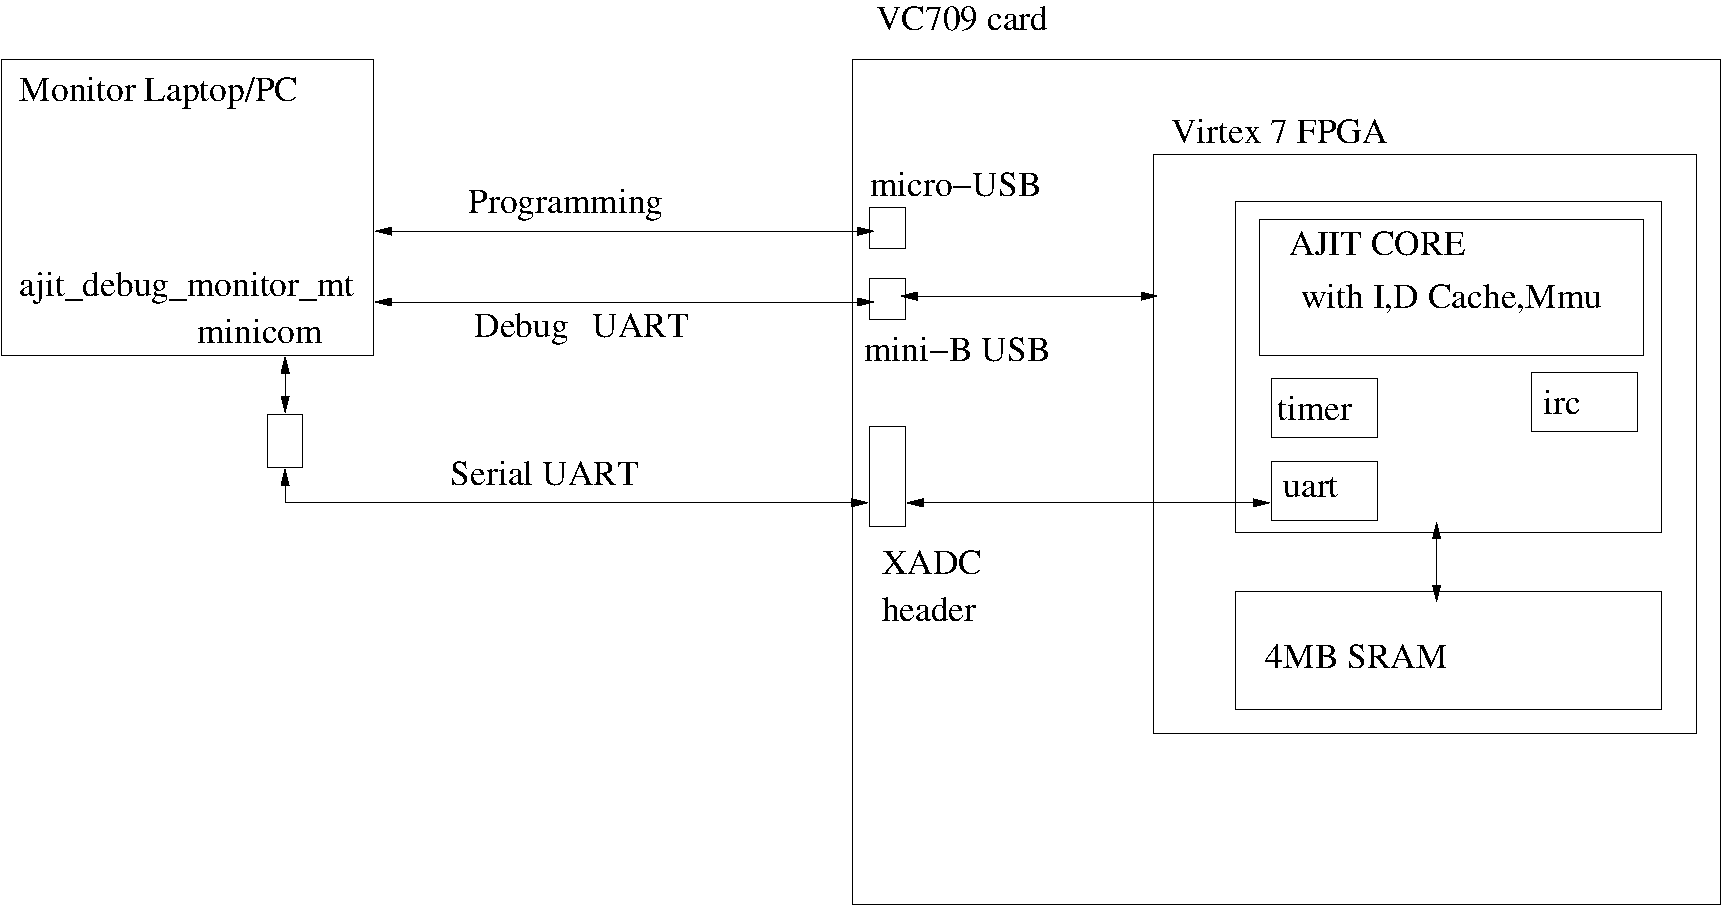
\includegraphics[width=10cm]{figs/vc709Setup.pdf}
  \caption{AJIT single board computer on VC709}
\end{figure}
}

\frame[containsverbatim]{\frametitle{Required Hardware}
\begin{itemize}
\item VC709 FPGA card.
\begin{itemize}
\item XADC connector must be mounted.
\end{itemize}
\item Micro-USB to USB cable.
\item Mini-B USB to USB cable.
\item Power cable for VC709.
\item UART CP210X.
\item Laptop/PC with at least 3 free USB slots.
\begin{itemize}
\item Running Linux.
\item We call this the monitor laptop.
\end{itemize}
\end{itemize}
}

\frame[containsverbatim]{\frametitle{Required Software}
\begin{itemize}
\item Latest AJIT Tool Chain, installed in monitor Laptop/PC.
\item Minicom terminal emulator.
\item Python-3.
\end{itemize}
}

\frame[containsverbatim]{\frametitle{Making the connections}
\begin{itemize}
\item Connect CP210X UART:
\begin{itemize}
\item CP210X Ground to XADC pin 16.
\item CP210X Tx  to  XADC pin 18 (GPIO-O).
\item CP210X Rx  to  XADC pin 17 (GPIO-1).
\item Note down USB tty id.  This will be used by the
serial device on the VC709.
\end{itemize}
\item Connect micro-USB cable between VC709 and monitor Laptop/PC.
\begin{itemize}
\item Note down the new USB tty ids.  These are used for
programming the FPGA on the VC709.
\end{itemize}
\item Connect mini-B USB cable between VC709 and monitor Laptop/PC.
\begin{itemize}
\item Note down the new USB tty id.  This will be used by the
debug connection between the monitor Laptop/PC and the AJIT system
on the FPGA.
\end{itemize}
\end{itemize}
}

\frame[containsverbatim]{\frametitle{Preparing and compiling an application}
\begin{itemize}
\item Write your main application C source/headers in the usual way.
\begin{itemize}
\item Use the print and timer routines provided as part of the
AJIT tool-chain.
\end{itemize}
\item Write init.s assembly file to initialize stack for bare-metal
execution.
\item Prepare a linker script.
\item Compile your application using the compile script provided
by the AJIT tool-chain.
\begin{itemize}
\item Prepare a compile script to specify assembly files, C source files, include directories, compiler 
options, defines etc for the script.
\item Run the compile script: this produces a memory map (mmap) file, as well as object dump, elf etc.
\end{itemize}
\end{itemize}
}

\frame[containsverbatim]{\frametitle{Running the application: minicom}
\begin{itemize}
\item Start minicom on the monitor Laptop/PC.
\begin{verbatim}
minicom -s
\end{verbatim}
\item Set the TTY id (note: connection to CP210x discussion above).
\item Set the baud-rate to 115200.
\item Line-feed, carriage return, local echo, log-file as per your requirements.
\end{itemize}
}

\frame[containsverbatim]{\frametitle{Running the application: ajit\_debug\_monitor\_mt}
\begin{itemize}
\item Start ajit\_debug\_monitor\_mt:
\begin{verbatim}
ajit_debug_monitor_mt -u /dev/ttyUSBx
\end{verbatim}
Here the USBx corresponds to the debug connection (mini-B USB to USB) discussed above.
\item Go through the following sequence:
\begin{verbatim}
w rst 1
m application.mmap
w rst 0
\end{verbatim}
You should be able to see the output of your program in minicom.
\end{itemize}
}

\frame[containsverbatim]{\frametitle{Resources}
\begin{itemize}
\item The 
\begin{verbatim}
AjitToolChain/AjitPublicResources/ajit_access_routines_mt
\end{verbatim}
 folder contains useful
AJIT hardware access routines.
\item The 
\begin{verbatim}
AjitToolChain/AjitPublicResources/minimal_printf_timer
\end{verbatim}
folder contains print and timer routines.
\end{itemize}
}

\frame[containsverbatim]{\frametitle{Dhrystone}
\begin{itemize}
\item Examine linker script.
\item Examine code.
\item Examine init.s file.
\item Examine compile script.
\item Run compile script.
\item Examine compile results.
\item Run the program.
\end{itemize}
}

\frame[containsverbatim]{\frametitle{Dhrystone linker script}
\begin{verbatim}
/*========================================================*/
/*                                                        */
/* Linker script for AJIT platform			  */
/*                                                        */
/*========================================================*/
ENTRY(_start)
SECTIONS
{
	. = 0x0;
	.text ALIGN(8) : { *(.text.main) *(.text*) }
	. = 0x10000;
	.rodata ALIGN(8) : { *(.rodata) }
}
\end{verbatim}
}


\frame[containsverbatim]{\frametitle{Dhrystone init.s file}
\begin{verbatim}
.global main
main:
_start:
	set 0xffe0f000, %sp  ! stack
	set 0xffe0f000, %fp  ! frame
	
	! mmu control register format
	!   [8]                    [7:1]  
        !   default-cacheable bit, unused
        !
	! mark all accesses as cacheable..
	!  (do not use without justification)
	!
	set 0x100, %o0
	sta %o0, [%g0] 0x4      

	! no arguments..
	call ajit_main
	nop
\end{verbatim}
}

\frame[containsverbatim]{\frametitle{Dhrystone unified.c file}
\begin{itemize}
\item Need to supply a timer routine
\begin{itemize}
\item ajit\_barebones\_clock returns ticks at clock\_frequency/256.
\end{itemize}
\item Need to supply a print routine
\begin{itemize}
\item ee\_printf.
\item Need to enable serial device.
\end{itemize}
\end{itemize}
}

\frame[containsverbatim]{\frametitle{Compile script}
\begin{itemize}
\item init.s file (Note: for this example, no trap handlers were supplied).
\item unified.c
\item AJIT access routines.
\item Minimal printf, timer.
\item uclibc.
\end{itemize}
}

\frame[containsverbatim]{\frametitle{Next steps}
\begin{itemize}
\item Trap handlers.
\item Using GDB with the AJIT single board computer.
\item Setting up a virtual to physical memory map while compiling your application.
\item Writing and using interrupt service routines.
\end{itemize}
}

\end{document}


